\documentclass[12pt]{article}
\usepackage[utf8]{inputenc}
\usepackage{graphicx}
\usepackage{amsmath}
\usepackage{hyperref}
\usepackage[margin=1in]{geometry}
\usepackage{listings}

% Configure listings package for Python
\lstset{
    language=Python,
    basicstyle=\ttfamily\small,
    numbers=left,
    numberstyle=\tiny\color{gray},
    frame=single,
    framesep=5pt,
    breaklines=true,
    showstringspaces=false,
    keywordstyle=\color{blue},
    identifierstyle=\color{black},
    stringstyle=\color{red},
    commentstyle=\color{green!50!black},
    rulecolor=\color{black},
    backgroundcolor=\color{gray!10},
    tabsize=4,
    captionpos=b,
    breakatwhitespace=false,
    escapeinside={\%*}{*}
}

\title{EE604 - Assignment 1}
\author{Lohit P Talavar}
\date{September 26, 2025}

\begin{document}

\maketitle

\section*{Introduction}
This report details the solutions for Assignment 1 of EE604, covering two main problems: text-to-image generation and image manipulation for removing leopard spots.

\section*{Q1: Text-to-Image Generation}
\subsection*{Problem Description}
The task was to develop a system that converts a given text input into an image. The system should support uppercase English letters (A-Z), space, basic punctuation (., ! ?), and newline characters. The rendering must be done using a simple bitmap font and pixel-level operations, without relying on built-in text-to-image conversion libraries.

\subsection*{Approach}
Our approach involved creating a custom bitmap font, where each supported character is represented as an $8 \times 6$ NumPy array (matrix) of $0$s and $1$s. A '$1$' indicates a pixel to be drawn (black), and '$0$' represents the background (white).

The `text_to_image` function processes the input text line by line. For each character in a line, it retrieves its corresponding bitmap from the `BITMAP_FONT` dictionary. It then iterates through the pixels of this bitmap and sets the corresponding pixels on a white canvas (a NumPy array) to black. Padding is added around the text to ensure readability. The final output is a grayscale image representing the rendered text.

\subsection*{Code}
Below is the Python code for the text-to-image generation system (`a.py`).
\lstinputlisting[caption={Code for Text-to-Image Generation (`a.py`)},label={lst:a_py}]{a.py}

\subsection*{Results}
The system successfully renders the input text into an image. An example output is shown in Figure \ref{fig:text_to_image}.

\begin{figure}[h!]
    \centering
    \includegraphics[width=0.8\textwidth]{Figure1.png} % Assuming Figure1.png is the output of a.py
    \caption{Output of the text-to-image generation system (Figure1).}
    \label{fig:text_to_image}
\end{figure}

\section*{Q2: Leopard Spot Removal}
\subsection*{Problem Description}
The objective was to remove the stripes (leopard spots) from a provided image. This is an image manipulation task requiring techniques to identify and then remove specific patterns from an image.

\subsection*{Approach}
The `remove_leopard_spots` function implements the solution.
\begin{enumerate}
    \item \textbf{Image Loading and Preprocessing:} The input image is loaded and converted to the HSV (Hue, Saturation, Value) color space. HSV is often preferred for color-based segmentation as it separates color information (Hue and Saturation) from brightness (Value), making it easier to isolate specific color ranges.
    \item \textbf{Spot Mask Creation:} A critical step is to create a mask that accurately identifies the leopard spots. This is achieved by defining a range of HSV values that correspond to the dark brown/black color of the spots. The `cv2.inRange` function is used to create a binary mask where pixels within this range are marked as white (potential spots) and others as black.
    \item \textbf{Mask Refinement (Morphological Operations):} To improve the mask's quality for inpainting, morphological operations are applied. Dilation (`cv2.dilate`) is used to slightly expand the identified spot regions. This ensures that the inpainting process covers the entire spot and its immediate edges, preventing artifacts.
    \item \textbf{Inpainting:} Finally, the `cv2.inpaint` function is used to fill the masked areas. This function reconstructs the masked region from the surrounding unmasked pixels. The `cv2.INPAINT_TELEA` method is chosen for its effectiveness in natural images, producing seamless reconstructions.
\end{enumerate}

\subsection*{Code}
Below is the Python code for the leopard spot removal system (`b.py`).
\lstinputlisting[caption={Code for Leopard Spot Removal (`b.py`)},label={lst:b_py}]{b.py}

\subsection*{Results}
The input image for the leopard spot removal task is shown in Figure \ref{fig:input_image_q2}. The process effectively identifies and removes the leopard spots, resulting in a cleaner image. The original input image, the generated spot mask, and the final inpainted image are shown in Figure \ref{fig:leopard_spot_removal}.

\begin{figure}[h!]
    \centering
    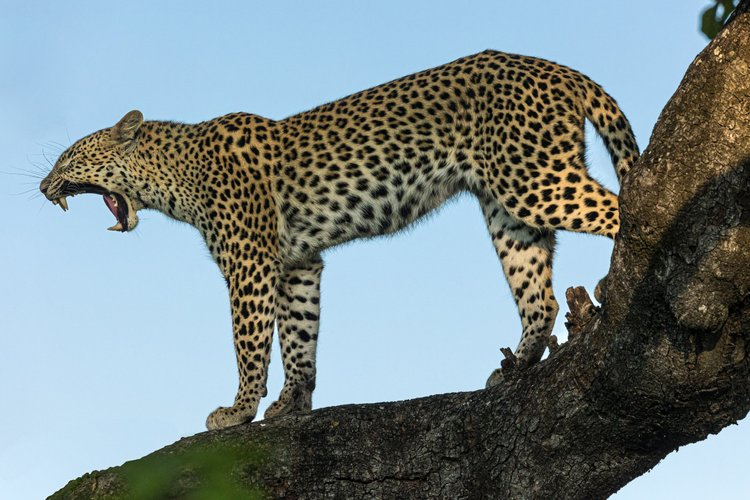
\includegraphics[width=0.6\textwidth]{image.jpg} % The input image for Q2
    \caption{Input image for the leopard spot removal task (Figure2).}
    \label{fig:input_image_q2}
\end{figure}

\begin{figure}[h!]
    \centering
    \includegraphics[width=0.9\textwidth]{Figure2.png} % Assuming Figure2.png is the output of b.py, which includes the original image
    \caption{Leopard spot removal process: Original input image, identified spots mask, and inpainted image (Figure3).}
    \label{fig:leopard_spot_removal}
\end{figure}

\section*{Conclusion}
This assignment successfully demonstrated the implementation of a custom text-to-image rendering system and an image processing pipeline for removing specific patterns using HSV color segmentation and inpainting.

\end{document}